\section{Semantic Segmentation with Convolutional Neural Network}
\label{sec:network}
\todo[inline]{Suggested subsections listed below}

\subsection{Patch-based architecture}
\todo[inline]{Outline what this thing actually predict. Patch based approach}
\todo[inline]{Input bigger than output. Context, etc}
\todo[inline]{Explain layering etc. show image}

\begin{figure}
\begin{center}
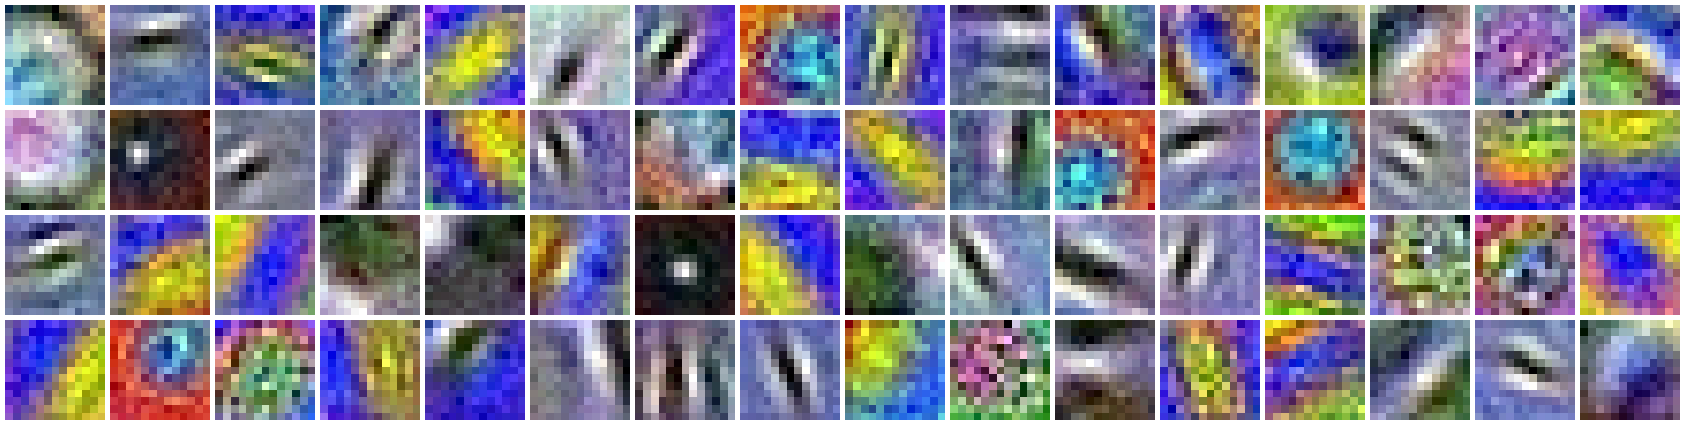
\includegraphics[width=1\columnwidth]{figs/network/Filter_unblurred.png}
\caption[Visualization of filter map]{Visualization of filter maps from the first convolutional layer of a trained network.}
\label{fig:convoluional_first_layer_visualization}
\end{center}
\end{figure}

\subsection{Optimization}
\todo[inline]{Sdg nesterov}
\subsection{Regularization}
\todo[inline]{Dropout}
\todo[inline]{L2 regularization}
\todo[inline]{Early stopping}
\todo[inline]{Leaky ReLu}

\subsection{Data preprocessing}
\todo[inline]{Rotation of aerial images}
\todo[inline]{Contrast normalization}
\todo[inline]{Flipping vertical|horizontal}
\todo[inline]{Class normalization. 50/50}




The system is based on the deep neural network outlined by \cite{Mnih_aerial_images_noisy}. The network have three convolutional layers and two fully connected layers. This network architecture is depicted in Figure \ref{fig:conv}. After the network is trained, it can predict whether or not roads are present in a $16 \times 16$ pixel area contained in the center of a $64 \times 64$ aerial image patch. The input patch is considerably larger than the output patch, so that the network can better utilize the context in the image. \\

The first layer perform convolution using $13 \times 13$ kernels, and outputs in total 64 feature maps. Only the first layer utilize max pooling, which reduces the number of inputs to the next layer as well as introducing some translational invariance to the model. The kernel size in the second and third layer are currently $4 \times 4$ and $3 \times 3$, respectably. The output of the third convolutional layer is used as input to a fully connected neural network with a single hidden layer and an output layer. The latter contains 256 units where each output is the probability of a pixel representing a road.\\

To avoid overfitting the training data, and hopefully achieve better generalization, different regularization schemes are applied during optimization, such as L2 weight decay, early stopping, and dropout. The first applies a weight penalty to prevent weights from growing large. The second stops the optimization process when performance on the validation set starts to consistently decrease. This is an indication of the model starting to overfit the training set. Dropout forces the units to rely less on each other, by randomly disabling half of the units in the network during training. This encourage units to encode independently useful information, since dropout penalize co-adaptation between units.\\

\todo[inline]{Talk about nesterov sgd, and mention RMSProp and regular prop supported via config}
The model parameters are optimized with a special form of \ac{SGD}, called RMSProp. RMSProp keeps a running average of the gradient magnitude for every weight which is used to adaptively adjust the learning rate of each weight. Compared to \ac{SGD}, this will result in a faster convergence. Other optimizers, such as Nesterov momentum, have also been implemented.\\ 

Before training occurs, a patch dataset suitable for the model is constructed. Each data and label image is rotated by a random amount, and a predefined number of image and label patches are extracted from the images. Before adding the sample to the training set, contrast normalization is applied. The mean pixel value in a patch is subtracted from each pixel, and divided by the standard deviation found for all pixels in the dataset.\\

\todo[inline]{Have to justify model layering. 256 output? why 64x64 input images why? Context. }
\todo[inline]{Large datasets, swap from memory to gpu (maybe)}